\PassOptionsToPackage{subsection=false}{beamerouterthememiniframes}
\PassOptionsToPackage{dvipsnames,table}{xcolor}
\documentclass[fleqn]{beamer}
\usepackage{graphicx}
\usepackage{multirow}
\usepackage{multicol}
\usepackage{amsmath,amsfonts,amsthm,amsopn}
\usepackage{color, colortbl}
\usepackage{subfig}
\usepackage{wrapfig}
\usepackage{fancybox}
\usepackage{tikz}
\usepackage{fancyhdr}
\usepackage{setspace}
\usepackage{xcolor}
\usepackage{movie15}
\usepackage{pifont}
\usepackage{soul}
\usepackage{fancyvrb,newverbs}
\usepackage{epsfig}
\usepackage{epstopdf}
\fvset{fontsize=\footnotesize}
\RecustomVerbatimEnvironment{verbatim}{Verbatim}{}

%\usepackage{fancybox}

\usetheme{Szeged}
\usecolortheme{default}

%\definecolor{links}{HTML}{2A1B81}
%\definecolor{links}{blue!20}
\hypersetup{colorlinks,linkcolor=,urlcolor=blue!80}

\setbeamertemplate{blocks}[rounded]
\setbeamercolor{block title}{bg=blue!40,fg=black}
\setbeamercolor{block body}{bg=blue!10}


\newenvironment<>{clicker}[1]{%
  \begin{actionenv}#2%
      \def\insertblocktitle{#1}%
      \par%
      \mode<presentation>{%
        \setbeamercolor{block title}{fg=white,bg=magenta}
       \setbeamercolor{block body}{fg=black,bg=magenta!10}
       \setbeamercolor{itemize item}{fg=magenta}
       \setbeamertemplate{itemize item}[triangle]
       \setbeamercolor{enumerate item}{fg=magenta}
     }%
      \usebeamertemplate{block begin}}
    {\par\usebeamertemplate{block end}\end{actionenv}}

%\newcommand{\bmp}{\begin{minipage}}
%\newcommand{\emp}{\end{minipage}}
%\newcommand{\blankcolumn}{\bmp{.05\textwidth}\hspace{0.50in} \emp}

\defbeamertemplate*{footline}{infolines theme}
{
  \leavevmode%
  \hbox{%
  \begin{beamercolorbox}[wd=.333333\paperwidth,ht=2.25ex,dp=1ex,left]{author in head/foot}%
    \usebeamerfont{author in head/foot}~~\insertshortinstitute: \insertshorttitle
  \end{beamercolorbox}%
  \begin{beamercolorbox}[wd=.67\paperwidth,ht=2.25ex,dp=1ex,right]{date in head/foot}%
    \usebeamerfont{date in head/foot}%\insertshortdate{}\hspace*{2em}
    \insertframenumber{} / \inserttotalframenumber\hspace*{2ex}
  \end{beamercolorbox}
  }%
  \vskip0pt%
}

\newcommand{\cmark}{\ding{51}}%
\newcommand{\xmark}{\ding{55}}%
\newcommand{\grp}{\textcolor{magenta}{Group Exercise}}
\newcommand{\grpc}{\textcolor{magenta}{Group Exercise, continued}}
\newcommand{\bsans}[1]{\underline{\hspace{0.2in}\color{blue!80}{#1}\hspace{0.2in}}}

\definecolor{cverbbg}{gray}{0.93}
\newenvironment{cverbatim}
 {\SaveVerbatim{cverb}}
 {\endSaveVerbatim
  \flushleft\fboxrule=0pt\fboxsep=.5em
  \colorbox{cverbbg}{\BUseVerbatim{cverb}}%
  \endflushleft
}
\newenvironment{lcverbatim}
 {\SaveVerbatim{cverb}}
 {\endSaveVerbatim
  \flushleft\fboxrule=0pt\fboxsep=.5em
  \colorbox{cverbbg}{%
    \makebox[\dimexpr\linewidth-2\fboxsep][l]{\BUseVerbatim{cverb}}%
  }
  \endflushleft
}

\newcommand{\bmp}{\begin{minipage}}
\newcommand{\emp}{\end{minipage}}
\newcommand{\blankcolumn}{\bmp{.05\textwidth}\hspace{0.50in} \emp}

 \newenvironment{code}[1]%
  {\vspace{.1in}\footnotesize\Verbatim[frame=single,label=SAS Code,commandchars=\\\{\},xrightmargin=#1\textwidth,framesep=.2in,labelposition=all]}
  {\endVerbatim\normalsize}

 \newenvironment{Rcode}[1]%
  {\vspace{.1in}\footnotesize\Verbatim[frame=single,label=R Code,commandchars=\\\{\},xrightmargin=#1\textwidth,framesep=.2in,labelposition=all]}
  {\endVerbatim\normalsize}

   \newenvironment{RcodeScript}[1]%
  {\vspace{.1in}\scriptsize\Verbatim[frame=single,label=R Code,commandchars=\\\{\},xrightmargin=#1\textwidth,framesep=.2in,labelposition=all]}
  {\endVerbatim\normalsize}

 \newenvironment{RcodeTiny}[1]%
  {\vspace{.1in}\tiny\Verbatim[frame=single,label=R Code,commandchars=\\\{\},xrightmargin=#1\textwidth,framesep=.2in,labelposition=all]}
  {\endVerbatim\normalsize}


   \newenvironment{Rout}[1]%
  {\vspace{.1in}\footnotesize\Verbatim[frame=single,label=R Output,commandchars=\\\{\},xrightmargin=#1\textwidth,framesep=.2in,labelposition=all]}
  {\endVerbatim\normalsize}
  
     \newenvironment{MTout}[1]%
  {\vspace{.1in}\footnotesize\Verbatim[frame=single,label=Minitab Output,commandchars=\\\{\},xrightmargin=#1\textwidth,framesep=.2in,labelposition=all]}
  {\endVerbatim\normalsize}

   \newenvironment{RoutScript}[1]%
  {\vspace{.1in}\scriptsize\Verbatim[frame=single,label=R Output,commandchars=\\\{\},xrightmargin=#1\textwidth,framesep=.2in,labelposition=all]}
  {\endVerbatim\normalsize}

 \newenvironment{RoutTiny}[1]%
  {\vspace{.1in}\tiny\Verbatim[frame=single,label=R Output,commandchars=\\\{\},xrightmargin=#1\textwidth,framesep=.2in,labelposition=all]}
  {\endVerbatim\normalsize}

\newenvironment{craw}[2]%
{\vspace{.1in}\footnotesize\Verbatim[frame=single,label=#2,commandchars=\\\{\},xrightmargin=#1\textwidth,framesep=.2in,labelposition=all]}
  {\endVerbatim\normalsize}


\newenvironment{scriptcraw}[2]%
{\vspace{.1in}\scriptsize \Verbatim[frame=single,label=#2,commandchars=\\\{\},xrightmargin=#1\textwidth,framesep=.2in,labelposition=all]}
  {\endVerbatim\normalsize}

  \newenvironment{tinycraw}[2]%
{\vspace{.1in}\tiny \Verbatim[frame=single,label=#2,commandchars=\\\{\},xrightmargin=#1\textwidth,framesep=.2in,labelposition=all]}
  {\endVerbatim\normalsize}




\title[Set 7]{Non-parametric methods: comparing groups}
\author[Pileggi]{Shannon Pileggi}

\institute[STAT 417]{STAT 417}

\date{}


\begin{document}

\begin{frame}
\titlepage
\end{frame}

\begin{frame}
\frametitle{OUTLINE\qquad\qquad\qquad} \tableofcontents[hideallsubsections]
\end{frame}


%===========================================================================================================================
\section[Getting started (2 groups)]{Getting started (2 groups)}
%===========================================================================================================================
\subsection{}

\begin{frame}
\frametitle{Comparing survival experiences of independent populations}
\hspace*{-0.3in}
\bmp{0.6\textwidth}
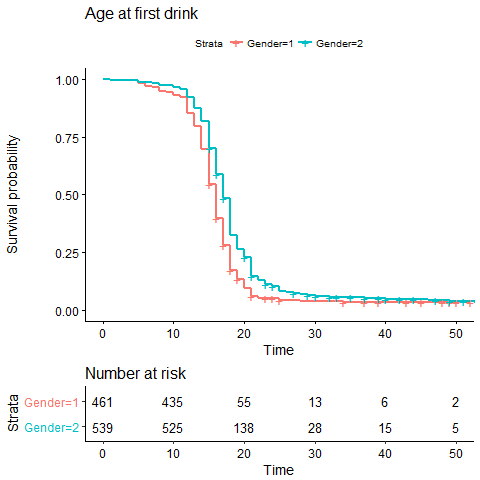
\includegraphics[width=1.0\textwidth]{Figures/KM_drink_gender.png}
\vskip200pt
\textcolor{white}{e}
\emp
\blankcolumn
\bmp{0.4\textwidth}
\small{
\begin{clicker}{\small{Which group appears to have the larger median survival time?}}
\begin{enumerate}
\item \texttt{1 = males}
\item \texttt{2 = females}
\end{enumerate}
\end{clicker}
\vskip2pt
Briefly comment on the survival experiences by gender.}
\vskip300pt
\textcolor{white}{e}
\emp
\end{frame}

\begin{frame}
\frametitle{Comparing survival experiences of independent populations}
The previous figure reveals an observed difference in the estimated survival curves among males and females based on the samples of ages.  Why can't we stop here?
\vskip300pt
\end{frame}

\begin{frame}
\frametitle{Inference procedures to compare survival experiences}
To compare survival curves over the range of time $t$ among several independent populations, we can conduct formal tests.:
\begin{enumerate}
\item
\item[]
\item
\item[]
\end{enumerate}
\end{frame}

\begin{frame}[fragile]
\frametitle{Age at first drink, by-hand example}
\begin{tabular}{l|lllllll}
Males & 43+ & 15 & 19 & 14 & 18+ & 16 & 14\\ \hline
Females & 18 & 15 & 17 & 16 & 40+ & 24+ & 16
\end{tabular}
\begin{Rcode}{-.05}
drinksub <- data.frame(time   = c(43, 15, 19, 14, 18, 16, 14,
                                  18, 15, 17, 16, 40, 24, 16),
                       censor = c( 0,  1,  1, 1,   0,  1,  1,
                                   1,  1,  1, 1,   0,  0,  1),
                       gender = c("m","m","m","m","m","m","m",
                                  "f","f","f","f","f","f","f"))

KM_obj <- survfit(Surv(time, censor) ~ gender, data = drinksub)

library(survminer)
ggsurvplot(KM_obj, data = drinksub,
           risk.table = TRUE,
           title = "Age at first drink (subset)")
\end{Rcode}
\end{frame}

\begin{frame}
\frametitle{Comparing survival experiences in \texttt{R}}
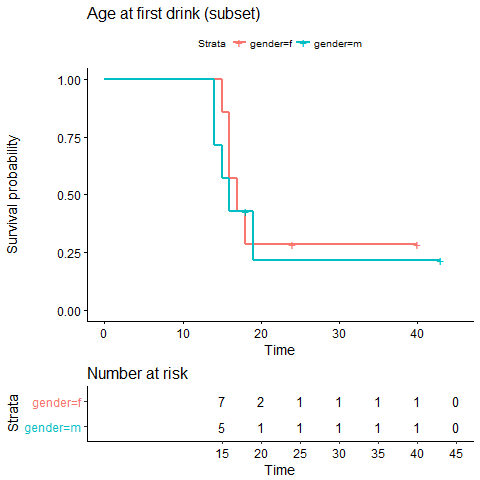
\includegraphics[width=0.70\textwidth]{Figures/KM_drinksub_gender.png}
\end{frame}

\begin{frame}
\frametitle{Comparing survival experiences in \texttt{Minitab}}
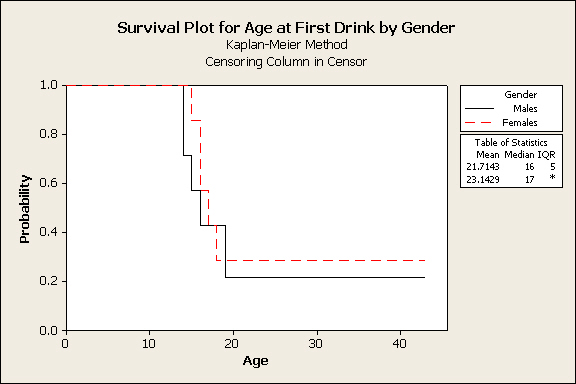
\includegraphics[width=0.70\textwidth]{Figures/km_gender_drink_sub_mt.jpg}
\end{frame}


\begin{frame}
\frametitle{Log-rank test}
The log-rank test can be used to compare survival experiences for \textbf{two} populations.  The general null and alternative hypotheses are:
\begin{itemize}
\item[]
\item[$H_0$:]
\item[]
\item[]
\item[]
\item[$H_a$:]
\item[]
\item[]
\item[]
\end{itemize}
\end{frame}

\begin{frame}
\frametitle{$H_0$ and $H_a$ for age at first drink}
In the age at first drink example, let \texttt{1 = males} and \texttt{2 = females}.  Then the null and alternative hypotheses are:
\begin{itemize}
\item[]
\item[$H_0$:]
\item[]
\item[]
\item[]
\item[$H_a$:]
\item[]
\item[]
\item[]
\end{itemize}
\end{frame}


%===========================================================================================================================
\section[Log-rank (2 groups)]{Log-rank (2 groups)}
%===========================================================================================================================
\subsection{}
\begin{frame}
\tableofcontents[currentsection, hideallsubsections]
\end{frame}

\begin{frame}
\frametitle{Log-rank test details}
The approach is to compare the total number of \textit{observed} events to the total number of \textit{expected} events in Group 1 under
 the assumption that $S_1(t)=S_2(t)$, where:
\begin{itemize}
\item $m$
\item[]
%the number of distinct ordered complete event times $t_{(1)}, t_{(2)}, \ldots, t_{(m)}$
%for both groups combined (we will not consider $t_{(0)}=0$ in our calculations).
\item $n_{1i}$
\item[]
%the number of subjects at risk of experiencing the event just prior to time
% $t_{(i)}$ in Group 1 only, for $i=1,\ldots,m$.
\item $n_{2i}$
%the number of subjects at risk of experiencing the event just prior to time $t_{(i)}$ in Group 2 only.
\item[]
\item $n_i=n_{1i}+n_{2i}$
\item[]
%the total number of individuals in both groups at risk just prior to time $t_{(i)}$
\item $d_{1i}$, $d_{2i}$, and $d_{i}$
\item[]
%are the observed number of event occurrences at each of the complete event times (in the interval
%starting at time $t_{(i)}$) for Group 1, Group 2, and the combined groups, respectively.
\end{itemize}
\end{frame}

\begin{frame}
\frametitle{Log-rank test details}
It is typically assumed that the number of event occurrences that will occur in time interval $i$, for Group 1 follows a \textit{hypergeometric} probability distribution.
%To find the expected number of event occurrences
%skip the details
\begin{itemize}
\item Let $d_i/n_i$ be the overall proportion of individuals at time $t_{(i)}$ who experience the event. Then the expected number of event occurrences in Group 1 at time $t_{(i)}$, denoted
$E_{1i}$, is given by:
\item[]
\item[]
\item Also, based on the assumption that the number of event
 occurrences at time $t_{(i)}$ for Group 1 follows a {hypergeometric} distribution,
the variance for the number of event occurrences for Group 1 at time $t_{(i)}$, denoted ${V}_{1i}$,
is given by:
\item[]
\item[]
%\begin{eqnarray}
%{V}_{1i} & = & \frac{n_{1i}n_{2i}d_i(n_i-d_i)}{n_i^2(n_i-1)}
%\nonumber
%\end{eqnarray}
\end{itemize}
\end{frame}

\begin{frame}[fragile]
\frametitle{Age at first drink, by-hand example}
\begin{tabular}{l|lllllll}
Males & 43+ & 15 & 19 & 14 & 18+ & 16 & 14\\ \hline
Females & 18 & 15 & 17 & 16 & 40+ & 24+ & 16
\end{tabular}
\vskip15pt
Write out the ordered event times:
\vskip5pt
%$\resizebox{1.0\textwidth}{!}{
{\renewcommand{\arraystretch}{2.5}
\begin{tabular}{|l|l|l|l|l|l|l|l|}
\hline
Order & ~~1~~  & ~~2~~ & ~~3~~ & ~~4~~ & ~~5~~ & ~~6~~ & ~~7~~ \\
\hline \hline
Males &  &  &  &  &  &  & \\
\hline
Females  &  &  &  &  &  &  & \\
\hline
\end{tabular}}
\end{frame}


\begin{frame}
\frametitle{Age at first drink, by-hand example}
\hspace*{-0.3in}
\resizebox{1.1\textwidth}{!}{
{\renewcommand{\arraystretch}{2.0}
\begin{tabular}{|c|c|c|c|c|c|c|c|c|c|c|}
\hline
$i$ & $~t_{(i)}~$ & Interval & $n_i$& $~d_i~$& $~~d_i/n_i~~$ & $~n_{1i}~$ & $~d_{1i}~$ & $~~n_{2i}~~$ & $~~{E}_{1i}~~$ & $~~{V}_{1i}~~$\\
\hline \hline
0&  & $[0,14)$ &  & & & & & & & \\
\hline
1&  & $[14,15)$ &  & & & & & & & \\
\hline
2&  & $[15,16)$ &  & & & & & & & \\
\hline
3&  & $[16,17)$ &  & & & & & & & \\
\hline
4&  & $[17,18)$ &  & & & & & & & \\
\hline
5&  & $[18,19)$ &  & & & & & & & \\
\hline
6&  & $[19,43)$ &  & & & & & & & \\
\hline
\end{tabular}}}
\end{frame}

\begin{frame}
\frametitle{Example calculations}
\begin{itemize}
\item[$E_{11}$:]
\item[]
\item[]
\item[]
\item[]
\item[$V_{11}$:]
\item[]
\item[]
\item[]
\item[]
\end{itemize}
\end{frame}

\begin{frame}
\frametitle{Log-rank test details}
\begin{itemize}
\item[] We compare the total observed and total expected counts over \textit{all} the
complete event times with the statistic:
% so we compare the sum of the observed event occurrences, $\sum_{i=1}^md_{1i}$, and
%the sum of the expected event occurrences, $\sum_{i=1}^mE_{1i}$, over all $m$ complete event times.
\item[]
\item[]
\item[]$\displaystyle \frac{observed - expected}{sd} = $
\item[]
\item[]
%\begin{eqnarray}
%\frac{\sum_{i=1}^m d_{1i}-\sum_{i=1}^mE_{1i}}{\sqrt{\sum_{i=1}^mV_{1i}}} \nonumber
%\end{eqnarray}

\item $\sum_{i=1}^md_{1i}$ is the sum of the observed event occurrences
\item $\sum_{i=1}^mE_{1i}$ is the sum of the expected event occurrences
\item $\sum_{i=1}^mV_{1i}$ is the variance of the total number of event occurrences over the $m$ complete event times

\end{itemize}
\end{frame}


\begin{frame}
\frametitle{Log-rank test details}
\begin{itemize}
\item This quantity is essentially a $z$-score, i.e:
\item[]
\item[]
\item[]
\item[]
\item[]
%it tells
%us how many standard deviations the total observed number of event occurrences is above or
%below its mean.
\item By the Central Limit Theorem, when each sample size $n_i$ is ``reasonably large," the above term
follows approximately a standard normal distribution.
\end{itemize}
\end{frame}


\begin{frame}
\frametitle{Log-rank test details}
\begin{itemize}
\item It is more common to see the square of the statistic reported in statistical software.

\item The square of the above statistic is called the \textbf{log-rank test statistic} (for two groups)
given by:
\item[]
\item[]
\item[]
\item[]
\item[]
\item[]
%\begin{eqnarray}
%\boxed{X_L^2= \frac{\left(\sum_{i=1}^m d_{1i}-\sum_{i=1}^mE_{1i}\right)^2}{\sum_{i=1}^m {V}_{1i}}
%          =  \frac{\left[\sum_{i=1}^m( d_{1i}-E_{1i})\right]^2}{\sum_{i=1}^m {V}_{1i}} } \nonumber
%\end{eqnarray}

\item This test statistic follows a \textbf{chi-square distribution} with 1
degree of freedom.


%thus we will reject $H_0:S_1(t)=S_2(t)$ and conclude the two
%population survival functions are significantly different.
\end{itemize}
\end{frame}

\begin{frame}
\frametitle{Discussion}
If the observed and expected number of events are far apart, then
\begin{itemize}
\item[]
\item $\chi^2_L$ will be \underline{(``big'', ``small'')},
\item[]
\item the corresponding $p$-value will be \underline{(``big'', ``small'')},
\item[]
\item leading to \underline{(evidence / no evidence)} to reject $H_0$.
\item[]
\end{itemize}
\end{frame}

\begin{frame}
\frametitle{Age at first drink, by-hand example}
Calculate the value of the log-rank test statistic:
\vskip300pt
\end{frame}

%===========================================================================================================================
\section[Software output (2 groups)]{Software output (2 groups)}
%===========================================================================================================================
\subsection{}
\begin{frame}
\tableofcontents[currentsection, hideallsubsections]
\end{frame}

\begin{frame}[fragile]
\frametitle{Minitab output}
\begin{MTout}{.3}
    ...
    Test Statistics

    Method    Chi-Square  DF  P-Value
    Log-Rank    0.131114   1    0.717
    Wilcoxon    0.425355   1    0.514
\end{MTout}
Conclusion?
\vskip300pt
\end{frame}

\begin{frame}
\frametitle{Wilcoxon test}
\begin{itemize}
\item The log-rank test statistic can be considered a special case of the following statistic:
\item[]
\item[]
\item[]
\item[]
%\begin{eqnarray}
%{\frac{\left[\sum_{i=1}^mw_i( d_{1i}-E_{1i})\right]^2}{\sum_{i=1}^m w_i^2{V}_{1i}} } \nonumber
%\end{eqnarray}
\item[] where the $w_i$'s are ``weights" all equal to \underline{\hspace{0.5in}}. %1
\item The \textbf{Wilcoxon test statistic}, denoted $X_W^2$, is also a special case of above statistic with  weights $w_i = n_i$, i.e:
\item[]
   \begin{eqnarray}
    X_W^2=\frac{\left[\sum_{i=1}^mn_i( d_{1i}-E_{1i})\right]^2}{\sum_{i=1}^m n_i^2{V}_{1i}}  \nonumber
    \end{eqnarray}
\item[] where $n_i$ is the number of subjects at risk just prior to time $t_{(i)}$
\item The {Wilcoxon test statistic}, $X^2$, also follows a $\chi^2$-distribution with 1 degree of freedom.
\end{itemize}
\end{frame}

\begin{frame}
\frametitle{Wilcoxon test statistic}
Verify that the value of the Wilcoxon test statistics is 0.4253.
\vskip300pt
\end{frame}

\begin{frame}
\frametitle{Comparison of log-rank and Wilcoxon tests}
\begin{enumerate}
\item
\item[]
\item[]
\item[]
\item[]
\item
\item[]
\item[]
\item[]
\item
\item[]
\item[]
\item[]
\end{enumerate}
\end{frame}

\begin{frame}[fragile]
\frametitle{Example of conflicting test results}
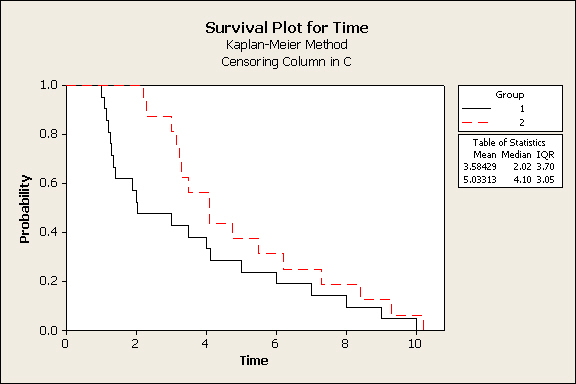
\includegraphics[width=0.70\textwidth]{Figures/ex_conflict_logrank_wilcoxon.jpg}\\
\begin{MTout}{.3}
Method    Chi-Square  DF  P-Value
Log-Rank     2.13966   1    0.144
Wilcoxon     4.27216   1    0.039
\end{MTout}
\end{frame}

\begin{frame}[fragile]
\frametitle{Log-rank test results in \texttt{R}}
\begin{Rcode}{-.05}
survdiff(Surv(time, censor) ~ gender, data = drinksub)
\end{Rcode}
\vskip5pt
\begin{Rout}{-.05}
Call:
survdiff(formula = Surv(time, censor) ~ gender, data = drinksub)

         N Observed Expected (O-E)^2/E (O-E)^2/V
gender=f 7        5     5.54    0.0523     0.131
gender=m 7        5     4.46    0.0649     0.131

 Chisq= 0.1  on 1 degrees of freedom, p= 0.717
\end{Rout}
\end{frame}

%===========================================================================================================================
\section[$>$ 2 groups]{$>$ 2 groups}
%===========================================================================================================================
\subsection{}
\begin{frame}
\tableofcontents[currentsection, hideallsubsections]
\end{frame}

\begin{frame}
\frametitle{Comparing survival experiences of $>2$ populations}
\begin{itemize}
\item The log-rank and Wilcoxon tests can easily be extended to $k>2$ populations.
\item The null and alternative hypotheses are now:
\begin{itemize}
\item[]
\item[$H_0$:]
\item[]
\item[]
\item[]
\item[]
\item[$H_a$:]
\item[]
\item[]
\item[]
\item[]
\end{itemize}

%\item Test statistic computations involve variance/covariance matrix calculations, so no mathematical details will be presented here. The distribution of the test statistic is:
\vskip .4in
% follows a $\chi^2$-distribution with $k-1$ degrees
%of freedom where $k=$number of groups.

%\item The extension of the log-rank test to more than two groups can be implemented in Minitab and \texttt{R}, while the Wilcoxon test can only be implemented in Minitab.
\end{itemize}
\end{frame}

\begin{frame}
\frametitle{Comparing survival experiences of $>2$ populations}
\begin{itemize}
\item Test statistic computations involve variance/covariance matrix calculations, so no mathematical details will be presented here. The distribution of the test statistic is:
\item[]
\item[]
\item[]
\item[]
% follows a $\chi^2$-distribution with $k-1$ degrees
%of freedom where $k=$number of groups.
\item The extension of the log-rank test to more than two groups can be implemented in Minitab and \texttt{R}, while the Wilcoxon test can only be implemented in Minitab.
\end{itemize}
\end{frame}

\begin{frame}
\frametitle{Lung cancer example (VALCSG)}
\small{
\begin{itemize}
\item There are two primary classifications of lung cancer based on the size and appearance of the malignant cells under a microscope: \textit{small cell} and \textit{non-small cell}.
\item \textbf{Small cell} lung cancer:  aggressive and spreads quickly through the body
\item Non-small cell lung cancer spreads more slowly and can be further sub-classified depending on origin and how the cells spread:
    \begin{itemize}
    \item \textbf{Squamous} cell carcinoma: Cancer that begins in squamous cells, which are thin, flat cells that look like fish scales.

    \item \textbf{Large cell} carcinoma: Cancer that may begin in several types of large cells.

    \item \textbf{Adenocarcinoma}: Cancer that begins in the cells that line the alveoli and make substances such as mucus
    \end{itemize}
\end{itemize}
%How do the survival experiences of patients with different types of lung cancer vary?
The Veterans Administration Lung Cancer Study Group (VALCSG) investigated the effects of two treatments (a standard treatment and test treatment) on the survival of patients.}
\end{frame}

\begin{frame}
\frametitle{Lung cancer example (VALCSG)}
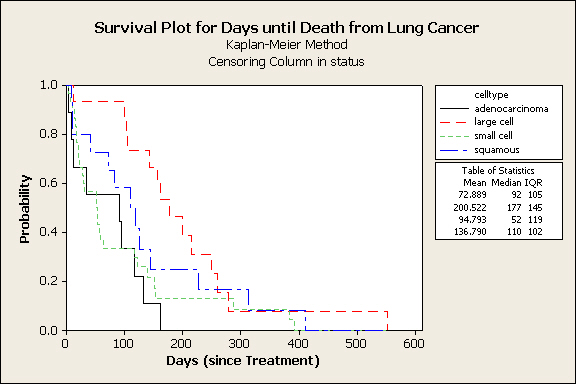
\includegraphics[width=0.7\textwidth]{Figures/km_valcsg.jpg}
\end{frame}


\begin{frame}[fragile]
\frametitle{Lung cancer example (VALCSG)}
\begin{MTout}{.3}
...
Test Statistics

Method    Chi-Square  DF  P-Value
Log-Rank      9.6408   3    0.022
Wilcoxon     11.5123   3    0.009
\end{MTout}
\begin{itemize}
\item[$H_0$:]
\item[]
\item[]
\item[]
\item[$H_a$:]
\item[]
\item[]
\item[]
\end{itemize}
\end{frame}


\begin{frame}
\frametitle{Lung cancer example (VALCSG)}
\begin{itemize}
\item State conclusion based on log-rank test at $\alpha = 0.01$.
\item[]
\item[]
\item[]
\item[]
\item[]
\item State conclusion based on Wilcoxon test at $\alpha = 0.01$.
\item[]
\item[]
\item[]
\item[]
\item[]
\end{itemize}
\end{frame}

\begin{frame}[fragile]
\frametitle{Lung cancer example (VALCSG) in \texttt{R}}
\begin{Rcode}{.0}
# focus on treatment group 1 only
veteran1 <- veteran[veteran$trt == 1, ]

KM_obj <- survfit(Surv(time, status) ~ celltype,
                  data = veteran1)

ggsurvplot(KM_obj, data = veteran1,
           risk.table = TRUE,
           title = "VALCSG study, trt=1")

survdiff(Surv(time, status) ~ celltype, data = veteran1)
\end{Rcode}
\end{frame}

\begin{frame}
\frametitle{Lung cancer example (VALCSG) in \texttt{R}}
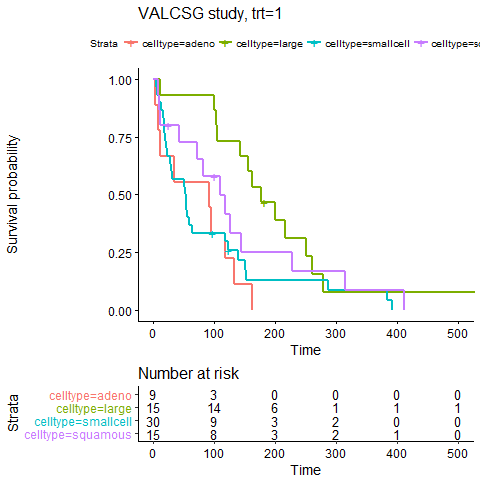
\includegraphics[width=0.7\textwidth]{Figures/KM_valcsg_r.png}
\end{frame}

\begin{frame}[fragile]
\frametitle{Lung cancer example (VALCSG) in \texttt{R}}
\hspace*{-0.2in}
\begin{Rout}{-.07}
Call:
survdiff(formula = Surv(time, status) ~ celltype, data = veteran1)

                    N Observed Expected (O-E)^2/E (O-E)^2/V
celltype=adeno      9        9     5.17     2.832     3.194
celltype=large     15       14    23.17     3.626     6.217
celltype=smallcell 30       28    21.14     2.225     3.503
celltype=squamous  15       13    14.52     0.159     0.211

 Chisq= 9.6  on 3 degrees of freedom, p= 0.0219
\end{Rout}
\end{frame}

\end{document} 